
\chapter{Notations en Algèbre spatiale} \label{appx_notations}

Les notations spécifiques à l'algèbre spatiale des torseurs permettent une formulation très simplifiée des relations cinématiques et dynamiques appliquées au \emph{modèle du système}.\\

\chapter{cachegrind - mesures de performance en vitesse d'exécution} \label{appx_cachegrind}

L'outil \textbf{cachegrind} est très efficace pour détecter des instructions ou blocs d'instructions très pénalisant pour la performance en vitesse d'un algorithme. Il s'agit d'un outil intégré à la boîte à outils Valgrind. L'outil permet de faire du profilage de fonctions. De plus, il existe un autre outil, \verb;Kcachegrind;, qui fournit une interface graphique permettant d'exploration ces données beaucoup plus facilement. Nous présentons rapidement ci-dessous son mode d'utilisation:
\begin{itemize}
\item[$\centerdot$ compilation du code source \emph{metapod}:] Il faut lancer la compilation avec les symboles de debug pour que \verb;Kcachegrind; puisse faire le lien entre les fonctions analysées et le code source correspondant.
\item[$\centerdot$ génération de l'analyse:]  \emph{callgrind} prend comme entrée l'exécutable de l'application à analyser et génère un seul fichier en sortie contenant toutes les données d'analyse ( \verb;callgrind.out.xxxxx; ). C'est le fichier à ouvrir avec \verb;Kcachegrind;.
\end{itemize}

Voici une capture écran de \verb;Kcachegrind; montrant une fenêtre où on peut visualiser l'ensemble des fonctions appelées par la fonction $BOOST$ "test\_chda". La taille des boîtes est proportionnelle au coût en temps d'exécution de la fonction associée:

\begin{figure}[H]
  \begin{center}
  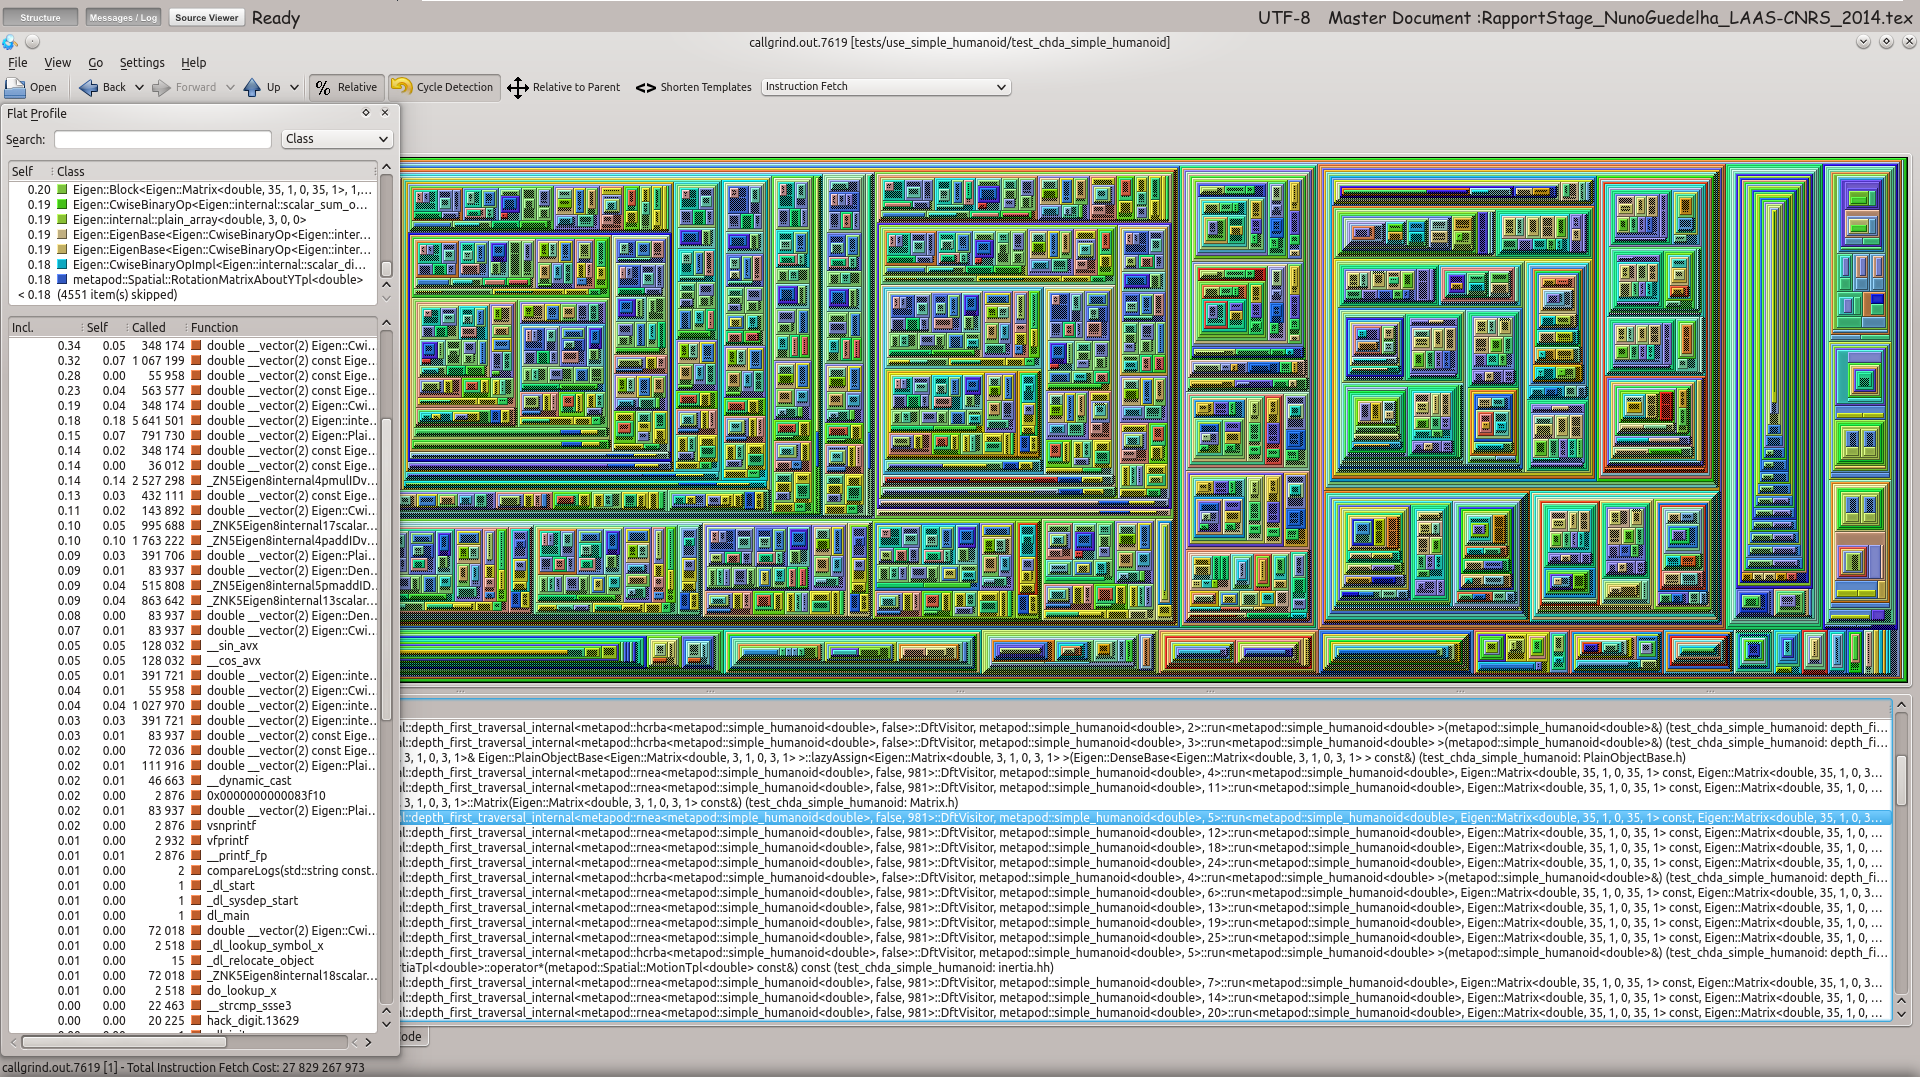
\includegraphics[width=\textwidth]{figs/snapshotKcachegrind1.png}
  \caption{Capture d'écran de Kcachegrind. Visualisation sous Kcachegrind du profil d'exécution des fonctions appelées par $test_chda$.}         % legende
  \label{fig:Kcachegrind1} % pour citer le numéro de figure
  \end{center}
\end{figure}



\chapter{Concepts et théorèmes en mécanique du solide à la base de l'algèbre spatiale} \label{appx_torseursToalgSpa}

\section{Les torseurs} \label{appx_torseursToalgSpa_torseurs}

\setmyFiguresFile{torseurs}

\subsection{Définition} \label{appx_torseursToalgSpa_torseurs_def}
Les théorèmes généraux de la dynamique des systèmes matériels mettent en jeux deux ensembles de vecteurs liés: celui des quantités de mouvement (cinématique) et celui des forces (dynamique). Ces ensembles n'interviennent que par les torseurs qui leur sont associés. On appelle torseur ($T$) l'ensemble d'un champ antisymétrique $M(A)$ et de son vecteur $S$. $M(A)$ et $S$ sont appelés respectivement \emph{moment} et \emph{vecteur} du torseur $[T]$.

\vspace{0.3cm} % retour à la ligne

\minipages[2]{c}
{.3}{.7}{}
{%
\begin{equation*}
[\underline{T}]=
\begin{bmatrix}
  \underline{S} \\
  \underline{M}(O)
\end{bmatrix}
\end{equation*}
}
{%
\begin{equation}
M(A)=M(B)+AB \times S \textnormal{ ou } M(B)=M(A)+S \times AB
\end{equation}
}
{}

\vspace{0.3cm} % retour à la ligne

Le champ antisymétrique en question n'est pas forcément un champ de vecteurs liés. C'est le cas, par exemple, du torseur cinématique d'un corps rigide en mouvement, constitué à partir du champ antisymétrique des vitesses du solide (vitesse d'un point du solide coïncidant avec un point fixe de l'espace). nous développons ce point dans la section \ref{appx_torseursToalgSpa_torseurs_appl}.

\subsection{Propriétés} \label{appx_torseursToalgSpa_torseurs_prop}

Nous regroupons dans cette section les propriétés des torseurs qui sont directement héritées et utilisées en algèbre spatiale.

\begin{flushleft}
\begin{spacing}{1.5}
\begin{tabular}{ l l c p{5cm} }
  \textbf{\textsc{é}galité:}
  & $[T_{1}]=[T_{2}]$ & $\implies$ & $\mathbf{S}_{1}=\mathbf{S}_{2} \textnormal{ et } \mathbf{M}_{1}(A)=\mathbf{M}_{2}(A)$ \\
  \textbf{Somme:}
  & $[T]=[T_{1}]+[T_{2}]$ & $\implies$ & $\mathbf{S}=\mathbf{S}_{1}+\mathbf{S}_{2} \textnormal{ et } \mathbf{M}(A)=\mathbf{M}_{1}(A)+\mathbf{M}_{2}(A)$ \\
  \textbf{Multiplication par un scalaire:}
  & $[T_{1}]=\lambda [T_{2}]$ & $\implies$ & $\mathbf{S}_{1}=\lambda \mathbf{S}_{2} \textnormal{ et } \mathbf{M}_{1}(A)=\lambda \mathbf{M}_{2}(A)$ \\
  \textbf{Torseur nul:}
  & \multicolumn{3}{l}{$\mathbf{S}=0 \textnormal{ et } \mathbf{M}(A)=0$} \\
  \textbf{Produit scalaire:}
  & $si [F]={\mathbf{F},\mathbf{M}(A)} \textnormal{ et } [v]={\mathbf{w},\mathbf{V}(A)}$ & $\implies$ & $[F][v] = \mathbf{F} \cdot \mathbf{v}(A) + \mathbf{M}(A) \cdot \mathbf{w}$ \\
  \textbf{Invariants:}
  & \multicolumn{3}{l}{(équiprojectivité) la projection de $\mathbf{M}$ sur $\mathbf{S}$} \\
  & \multicolumn{3}{l}{(équiprojectivité) la projection de $\mathbf{M}$ sur $\mathbf{AB}$} \\
  & \multicolumn{3}{l}{Le produit scalaire $[F][v]$.} \\
  \multicolumn{1}{p{6cm}}{\textbf{Torseur lié à un ensemble de vecteurs liés:}}
  & \multicolumn{3}{p{10cm}}{Le moment d'un ensemble de vecteurs liés ${(A_{i},\mathbf{V}_{i})}$ a la forme d'un champ antisymétrique \cite{bib_champVecteurs} (chapitre IV). On lui associe donc
  le torseur} \\
  & \multicolumn{3}{l}{$\mathbf{S}=\Sigma_{i}\mathbf{V}_{i} (\emph{vecteur}) \textnormal{ et } \mathbf{M}(O)=\Sigma_{i}\mathbf{OA}_{i} \times \mathbf{V}_{i} (\emph{moment}).$} \\
\end{tabular}
\end{spacing}
\end{flushleft}

%Fixe la largeur de la 1ere colonne
%\newlength{\my1rstColumnWidth}
%\settowidth{\my1rstColumnWidth}{Multiplication par un scalaire:}
%\setlength{\my1rstColumnWidth}{.5in}

Remarque: on appelle invariants d'un torseur les quantités qui restent constantes quelque soit le point fixe dans l'espace où ce torseur est définit.

\subsection{applications} \label{appx_torseursToalgSpa_torseurs_appl}

\subparagraph{Torseur-vitesse:}

Dans l'étude de la dynamique des systèmes matériels, le champ de vitesses d'un corps rigide en mouvement \footnote{on se limite ici au cas des corps rigides} a la forme d'un champ antisymétrique (vecteurs non liés au corps), et son vecteur $\mathbf{w}$ définit la vitesse angulaire de rotation du solide. On lui associe donc un torseur dont les éléments de réduction sont:

\minipages[2]{|c}
{.75}{.4}{}
{%
\medskip
\begin{description}
  \item[vecteur $\mathbf{S}$:] vitesse angulaire $\mathbf{\omega}$ autour de l'axe de rotation considéré passant par $O$
  \item[moment $\mathbf{M}(O)$:] vitesse linéaire $\mathbf{v}(O)$ du solide au point $O$
\end{description}
\medskip
}{%
\\
\begin{tabular}{|r}
\(
\widehat{\underline{v}}_O=
\begin{bmatrix}
  \mathbf{\underline{S}}    \\
  \mathbf{\underline{M}}(O)
\end{bmatrix}
=
\begin{bmatrix}
  \mathbf{\underline{\omega}} \\
  \mathbf{\underline{v}}_O
\end{bmatrix}
\)
\end{tabular}
\medskip
}
{}

Et on peut exprimer la vitesse de deux points quelconques $A$ et $B$ liés au solide, par rapport à un repère fixe $R$, sous la forme:

\begin{equation}
\mathbf{v}_{B/\emph{R}}=\mathbf{v}_{A/\emph{R}}+\mathbf{BA} \times w_{S/\emph{R}}
\end{equation}
Nous retrouvons ici la forme de la vitesse spatiale établie dans la section \ref{algSpa_Vitesse}.

\subparagraph{Torseur cinétique:}

Le centre de masse $C$ d'un solide quelconque est défini par:
\begin{equation}
\mathbf{OC} = \frac{1}{M} \int_\vartheta \! \mathbf{OA}\rho \mathrm{d} \vartheta
\end{equation}
Où $\rho$ est la masse volumique, $\vartheta$ le volume total du corps rigide et $M$ sa masse totale. La quantité de mouvement $\mathbf{P}$ se calcule en intégrant les quantités de mouvement élémentaires $v \mathrm{d}m$ sur tout le volume $\vartheta$:
\begin{equation}
\mathbf{P} = \int_\vartheta \mathbf{v} \mathrm{d}m = \int_\vartheta \rho \mathbf{v} \mathrm{d}v = M\mathbf{v}_{C}
\end{equation}
De même, le moment cinétique $\mathbf{L}_{O}$ ($O$ origine d'un repère fixe dans l'espace) se calcule en intégrant les moments cinétiques élémentaires sur tout le volume $\vartheta$. Il en résulte une relation simple entre les moments cinétiques en $O$ et un autre point quelconque fixe de $\mathcal{R}$, $O'$:
\begin{equation}\label{momentKantiSym}
\mathbf{L}_O = \int_\vartheta \mathbf{OA} \times \mathbf{v}_A \rho \mathrm{d} \vartheta \quad \textnormal{ et } \quad \mathbf{L}_O = \mathbf{OO'} \times \mathbf{P} + \mathbf{L}_{O'}
\end{equation}
De plus, le théorème de Koenig permet de relier les moments cinétiques $\mathbf{L}_O$ par rapport à $\mathcal{R}$ et $\mathbf{L}^*$ par rapportà  $\mathcal{R^*}$, $\mathcal{R^*}$ étant le repère où le centre de masse est fixe. Le calcul de $\mathbf{L}_O$ dans $\mathcal{R}$ est ainsi simplifié:
\[
\begin{alignedat}{2}
\mathbf{L}_C = \mathbf{L}^* \quad \implies \quad \mathbf{L}_O = \mathbf{OC} \times \mathbf{P} + \mathbf{L}^* \quad \textnormal{ avec } &\quad \mathbf{L}^* &&= \int_\vartheta \rho \mathbf{CA} \times \mathbf{v}^* \mathrm{d} \vartheta \\
\textnormal{(Pour un solide)} &\quad \mathbf{L}^* &&= [I]_C \mathbf{\omega}
\end{alignedat}
\]

\textbf{Remarque:} Dans le cas d'un solide $\mathcal{S}$ en rotation ayant un point fixe $O$ dans $\mathcal{R}$, le moment cinétique exprimé en $O$ est donné par 
\colorbox[gray]{0.8}{\( \mathbf{L}_{O/\mathcal{R}} = [I]_O \mathbf{\omega} \)}, 
où $\mathbf{\omega}$ est le vecteur rotation du solide et $[I]_O$ est l'opérateur d'inertie dans $\mathcal{R}$. Or le centre de masse $C$ de $\mathcal{S}$ est bien un point fixe de $\mathcal{R^*}$, donc on obtient \colorbox[gray]{0.8}{\( \mathbf{L^*} = \mathbf{L}_{C/\mathcal{R^*}} = [I]_C \mathbf{\omega} \)}.

La relation entre les moments cinétiques en deux points fixes $O$ et $O'$ étant antisymétrique \eqref{momentKantiSym}, on peut associer au système de vecteurs liés $\{\rho \mathbf{v}_A \mathrm{d}\vartheta\}$, le torseur $[P]$ dit \emph{torseur cinétique}:

\minipages[2]{|c}
{.6}{.6}{}
{%
\medskip
\begin{description}
\item[moment $\mathbf{M}(O)$:] moment cinétique  $\mathbf{L}_O$ du solide au point $O$
\item[vecteur $\mathbf{S}$:] quantité de mouvement du système $\mathbf{P}$
\end{description}
\medskip
}{%
\\
\begin{tabular}{|r}
\(
\widehat{\underline{P}}_O=
\begin{bmatrix}
  \mathbf{\underline{M}}(O) \\
  \mathbf{\underline{S}}
\end{bmatrix}
=
\begin{bmatrix}
  \mathbf{\underline{\mathbf{L}}}_O \\
  \mathbf{\underline{P}}
\end{bmatrix}
\)
\end{tabular}
\medskip
}
{}


\subparagraph{Torseur-force:}

nous considérons maintenant les forces appliquées au solide $\mathcal{S}_d$ (déformable dans le cas général), toujours en mouvement par rapport au référentiel $\mathcal{R}$. Soit le vecteur lié générique $(A,\mathbf{f}_v)$ représentant la force volumique appliquée à l'élément de matière de volume $\mathrm{d}\vartheta$ qui entoure $A$, un point fixe de $\mathcal{S}$ (figure \ref{fig_systemeDeForces.a}. Cette force inclut les forces extérieures à $\mathcal{S}_d$ ainsi que les forces exercées par les autres éléments de matière de $\mathcal{S}_d$. Notamment, si le référentiel n'est pas galiléen, il faut compter également les forces de Coréolis. On représente donc le système de forces appliquées à $\mathcal{S}_d$ par l'ensemble des vecteurs liés ${(A,\mathbf{f}_v\mathrm{d}\vartheta)}$, pour lequel on calcule la somme des forces et le moment (couple) résultant des forces $O$:

\begin{equation}
\mathbf{f} = \int_\vartheta \mathbf{f}_v\mathrm{d}\vartheta \textnormal{ et } \mathbf{n}_O = \int_\vartheta \mathbf{OA} \times \mathbf{f}_v\mathrm{d}\vartheta
\end{equation}

\dispThreeFig[H]
{1}{vecteur force volumique lié}
{2}{somme des forces et moment des forces}
{3}{Transformation: moment par rapport à un autre point $O'$}
{système de forces des vecteurs liés ${(A,\mathbf{f}_v\mathrm{d}\vartheta)}$}
{fig_systemeDeForces}

Dans cette représentation, on considère $S$ comme une force linéaire globale passant par $O$, avec son moment global $M$ en $O$ associé (figure \ref{fig_systemeDeForces.b}).
On calcule également la relation simple entre les moments des forces en $O$ et un autre point quelconque fixe de $\mathcal{R}$, $O'$ (figure \ref{fig_systemeDeForces.c}):
\begin{equation}\label{}
\mathbf{n}_O = \int_\vartheta (\mathbf{OO'} + \mathbf{O'A}) \times \mathbf{f}_v\mathrm{d}\vartheta = \mathbf{n}_{O'} + \mathbf{OO'} \times \mathbf{f}
\end{equation}

On peut donc associer au système de vecteurs liés ${(A,\mathbf{f}_v\mathrm{d}\vartheta)}$ le torseur $[F]$ dit \emph{torseur-force}:

\minipages[2]{|c}
{.7}{.6}{}
{%
\medskip
\begin{description}
\item[moment $\mathbf{M}(O)$:] couple résultant des forces $\mathbf{n}_O$ du solide au point $O$
\item[vecteur $\mathbf{S}$:] somme des forces du système $\mathbf{f}$
\end{description}
\medskip
}{%
\\
\begin{tabular}{|r}
\(
\widehat{\underline{f}}_O=
\begin{bmatrix}
  \mathbf{\underline{M}}(O) \\
  \mathbf{\underline{S}}
\end{bmatrix}
=
\begin{bmatrix}
  \mathbf{\underline{\mathbf{n}}}_O \\
  \mathbf{\underline{f}}
\end{bmatrix}
\)
\end{tabular}
\medskip
}
{}

Remarque: Les torseurs $\widehat{f}_O$ et $\widehat{f}_O'$ sont équivalents car ils décrivent les mêmes force/mouvement du centre de masse et couple autour du centre de masse du solide. Cette équivalence n'est pas forcément vraie pour l'ensemble du système de forces (par exemple le cas d'un ressort soit comprimé soit étiré par deux forces parallèles et opposées).


\subparagraph{Torseur dynamique:}

Comme pour la quantité de mouvement $P$ et le moment cinétique $L$, nous calculons la quantité d'accélération (somme dynamique) et le moment résultant de cette accélération (moment dynamique) en intégrant les grandeurs élémentaires respectives sur tout le volume, et nous montrons que:
\begin{align}
\mathbf{D} &= \int_\vartheta \mathbf{a} \mathrm{d}m = \frac{\mathrm{d}}{\mathrm{d}t} \int_\vartheta \mathbf{v} \mathrm{d}m = \frac{\mathrm{d}}{\mathrm{d}t} (M \mathbf{v}_{C}) \\
\mathbf{L}_O &= \int_\vartheta \mathbf{OA} \times \rho \mathbf{a}_A \mathrm{d} \vartheta \quad \textnormal{ et } \quad \mathbf{N}_O = \mathbf{OO'} \times \mathbf{D} + \mathbf{N}_{O'}
\end{align}
où $O'$ est un autre point fixe de $\mathcal{R}$.

\medskip

On peut donc associer au système de vecteurs liés ${(A,\rho \mathbf{a}_A \mathrm{d}\vartheta)}$ le torseur $[D]$ dit \emph{torseur dynamique}:

\minipages[2]{|c}
{.7}{.6}{}
{%
\medskip
\begin{description}
\item[moment $\mathbf{M}(O)$:] moment dynamique résultant $\mathbf{N}_O$ du solide au point $O$
\item[vecteur $\mathbf{S}$:] quantité d'accélération du centre de masse $\mathbf{D}$
\end{description}
\medskip
}{%
\\
\begin{tabular}{|r}
\(
\widehat{\underline{D}}_O=
\begin{bmatrix}
  \mathbf{\underline{M}}(O) \\
  \mathbf{\underline{S}}
\end{bmatrix}
=
\begin{bmatrix}
  \mathbf{\underline{\mathbf{N}}}_O \\
  \mathbf{\underline{D}}
\end{bmatrix}
\)
\end{tabular}
\medskip
}
{}



\chapter{Quelques démonstrations en algèbre spatiale} \label{appx_dem}

\setmyFiguresFile{figures}

\section{Invariance du vecteur spacial $\widehat{v}$}

\subsection{invariance entre deux bases de \emph{Plücker} ayant la même orientation}

Nous allons démontrer l'invariance du vecteur spatial dans le cas simple illustré ci-dessous:

\dispThreeFig[H]
{4}{Deux bases de \emph{Plücker} de même orientation.}
{5}{Expression de $\textbf{d}_{Py}$ et $\textbf{d}_{Pz}$ en $O$.}
{6}{cas de $\textbf{d}_{Pz}$ (projection suivant $\textbf{d}_{z}$).}
{Expression de $\textbf{d}_{Px}$, $\textbf{d}_{Py}$ et $\textbf{d}_{Pz}$ en $O$.}
{vitessePointCoincidant}

On considère les deux bases de \emph{Plücker}:

\begin{align*}
D_{O} = \lbrace &\textbf{d}_{Ox}, \textbf{d}_{Oy}, \textbf{d}_{Oy}, \textbf{d}_{x}, \textbf{d}_{y}, \textbf{d}_{z} \rbrace \\
D_{P} = \lbrace &\textbf{d}_{Px}, \textbf{d}_{Py}, \textbf{d}_{Py}, \textbf{d}_{x}, \textbf{d}_{y}, \textbf{d}_{z} \rbrace \\
\end{align*}

Dans la section \ref{algSpa_Vitesse}, figure \ref{fig_transPlucker}, nous avons montré la relation entre les vecteurs unitaires de mouvement des deux bases de \emph{Plücker} $D_{O}$ et $D_{P}$:

\begin{align*}
  \textbf{d}_{Px} &= \textbf{d}_{Ox} \\
  \textbf{d}_{Py} &= \textbf{d}_{Oy}+r \textbf{d}_{z} \\
  \textbf{d}_{Pz} &= \textbf{d}_{Oz}-r \textbf{d}_{y}
\end{align*}

On considère à présent un corps $C$ en translation et en rotation autour d'un axe quelconque dans l'espace. Le vecteur spatial $\widehat{v}$ de ce corps en $O$, s'exprime dans la base de \emph{Plücker} $D_{O}$ comme suit:

\begin{equation*}
  \widehat{v} = w_{x}\textbf{d}_{Ox} + w_{y}\textbf{d}_{Oy} + w_{z}\textbf{d}_{Oz} + v_{Ox}\textbf{d}_{x} + v_{Oy}\textbf{d}_{y} + v_{Oz}\textbf{d}_{z}
\end{equation*}

Le vecteur spatial $\widehat{v'}$ de ce corps en $P$, s'exprime dans la base de \emph{Plücker} $D_{P}$ comme suit:

\begin{equation*}
  \widehat{v'} = w_{x}\textbf{d}_{Px} + w_{y}\textbf{d}_{Py} + w_{z}\textbf{d}_{Pz} + v_{Px}\textbf{d}_{x} + v_{Py}\textbf{d}_{y} + v_{Pz}\textbf{d}_{z}
\end{equation*}

Nous voulons l'exprimer dans la base $D_{O}$. $w_{x}$, $w_{y}$ et $w_{z}$ sont connus. Calculons $v_{Px}$, $v_{Py}$ et $v_{Pz}$:

\vspace{0.3cm}
\minipages[2]{t}{.4}{.6}{}
{%
\(
\begin{alignedat}{3}
  & &&\phantom{xxx} v_{P} &&= v_{O} + w \times \overrightarrow{OP} \\
  \vspace{0.5cm}
  &\iff &&\phantom{xxx} \underline{v}_{P}
  &&=
  \underline{v}_{O}+\underline{w}\times
  \begin{bmatrix}
    r\\
    0\\
    0
  \end{bmatrix} \\
  \vspace{0.5cm}
  &\iff
  &&\begin{bmatrix}
    v_{Px} \\
    v_{Py} \\
    v_{Pz}
  \end{bmatrix}
  &&=
  \begin{bmatrix}
    v_{Ox}\\
    v_{Oy}+w_{z}r\\
    v_{Oz}-w_{y}r
  \end{bmatrix}
  \quad \texttt{or} \quad
  \widehat{\underline{v}'}
  =
  \begin{bmatrix}
    \underline{w} \\
    \underline{v}_{P}
  \end{bmatrix}
\end{alignedat}
\)}
{%
\begin{tabular}{|p{\textwidth}}
\(\begin{alignedat}{2}
  &\iff
  \widehat{v'} &&= w_{x}\textbf{d}_{Px} + w_{y}\textbf{d}_{Py} + w_{z}\textbf{d}_{Pz} \\
  &            &&\phantom{{}={}} + v_{Px}\textbf{d}_{x} + v_{Py}\textbf{d}_{y} + v_{Pz}\textbf{d}_{z} \\
  &            &&= w_{x}\textbf{d}_{Ox} + w_{y}(\textbf{d}_{Oy}+r\textbf{d}_{z}) + w_{z}(\textbf{d}_{Oz}-r\textbf{d}_{y}) \\
  &            &&\phantom{{}={}} + v_{Ox}\textbf{d}_{x} + (v_{Oy}+w_{z}r)\textbf{d}_{y} + (v_{Oz}-w_{y}r)\textbf{d}_{z} \\
  &            &&= w_{x}\textbf{d}_{Ox} + w_{y}\textbf{d}_{Oy} + w_{z}\textbf{d}_{Oz} + v_{Ox}\textbf{d}_{x} + v_{Oy}\textbf{d}_{y} + v_{Oz}\textbf{d}_{z} \\
  &            &&= \widehat{v}
\end{alignedat}\)
\end{tabular}
}
{}
\vspace{0.3cm}

Nous avons ainsi montré l'équivalence des deux vecturs spatiaux $\widehat{v}$ et $\widehat{v'}$.

\subsection{invariance entre deux bases de \emph{Plücker} quelconques et relation avec }


\chapter{\textsc{é}léments d'algèbre linéaire} \label{appx_algLineaire}




